% Copyright (C) Data Structures and Algorithms Team.
\chapter{Searching}

\section{Sequential Search}
A simple algorithm that search for a specific item inside a list. It operates looping on each element $O(n)$ until a match occurs or the end is reached.

\begin{tabbing}
1) \textbf{alg}\= \textbf{orithm} SequentialSearch($list$, $item$)\\
2) \> \textbf{Pre:}~~ $list~!=~\emptyset$ \\
3) \> \textbf{Post:}~ return $index$ of item if found, otherwise $-1$ \\
4) \> \= $index \leftarrow 0$ \\
5) \> \textbf{whi}\= \textbf{le} $index < list$.Count  \textbf{and} $list$[$index$]~!= $item$ \\
6) \> \> \= $index \leftarrow index+1$ \\
7) \> \textbf{end while} \\
8) \> \textbf{if }\= $ index < list$.Count  \textbf{and} $list$[$index$] = $item$ \\
9) \> \> \textbf{return} $index$ \\
10)\> \textbf{end if} \\
11)\> \textbf{return} $-1$ \\ 
12) \textbf{end} SequentialSearch \\

\end{tabbing}

\section{Probability Search}
Probability search is a statistical sequential searching algorithm. In addition to searching for an item, it takes into account its frequency by swapping it with it's predecessor in the list. The algorithm complexity still remains at $O(n)$ but in a non-uniform items search the more frequent items are in the first positions, reducing list scanning time.

Figure \ref{fig:search_seq} shows the resulting state of a list after searching for two items, notice how the searched items have had their search probability increased after each search operation respectively.

\newpage
\begin{tabbing}
1) \textbf{alg}\= \textbf{orithm} ProbabilitySearch($list$, $item$)\\
2) \> \textbf{Pre:}~~ $list~!=~\emptyset$ \\
3) \> \textbf{Post:}~ a boolean indicating where the item is found or not;\\
   \>~~~~~~~~~ in the former case swap founded item with its predecessor \\
4) \> \= $index \leftarrow 0$ \\
5) \> \textbf{whi}\= \textbf{le} $index < list$.Count  \textbf{and} $list$[$index$]~!= $item$ \\
6) \> \> \= $index \leftarrow index+1$ \\
7) \> \textbf{end while} \\
8) \> \textbf{if }\= $ index \geq list$.Count  \textbf{or} $list$[$index$] ~!= $item$ \\
9) \> \> \textbf{return} false \\
10)\> \textbf{end if} \\
11)\> \textbf{if }\= $ index > 0$ \\
12)\> \> $Swap(list[index], list[index-1])$ \\
13)\> \textbf{end if } \\
14)\> \textbf{return} true \\ 
15) \textbf{end} ProbabilitySearch \\
\end {tabbing}

\begin{figure}
\begin{center}
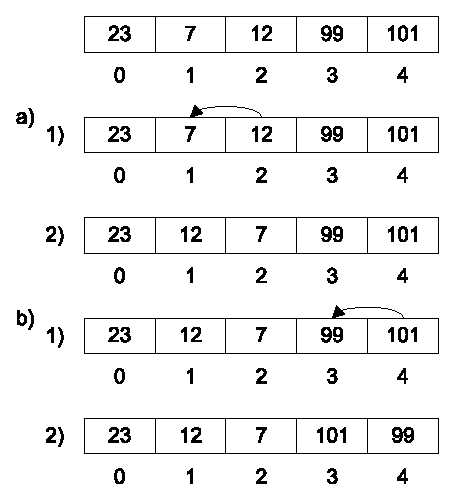
\includegraphics{search_sequential}
\end{center}
\caption{a) Search($12$), b) Search($101$)} \label{fig:search_seq}
\end{figure}
